
\documentclass[12pt]{article}
\usepackage[utf8]{inputenc}
\usepackage{listings}
\usepackage[margin=1in]{geometry}
\usepackage{graphicx} % graficos
\usepackage{setspace}
\usepackage{xcolor}
\usepackage{color}
\usepackage{indentfirst}
\usepackage{listings}
% \usepackage{isomath}
\usepackage{ulem}
\usepackage{caption}
\usepackage{algorithmicx}
\usepackage{algpseudocode}
\usepackage{algorithm}
% \algnewcommand{\LineComment}[1]{\State \(\triangleright\) #1}
\algnewcommand{\LineComment}[1]{\State \(\triangleright\) #1}
\usepackage{minted}
\usepackage{wasysym}




\begin{document}


\begin{titlepage}
\begin{center}
\vspace*{1.in}
\begin{Large}


{\huge  Trabajo Especial de Modelos y Simulación }


\vspace{2.5in}
{\it Lucas Alonso}\\
{\it Guillermo Incatasciato}

\vspace*{3in}


16 de Junio, 2017
\vspace*{0.5in}

FAMAF, UNC

\end{Large}
\end{center}
\end{titlepage}

\section{Introducción}
En este proyecto estudiaremos el {\it tiempo operativo} de un sistema a travéz de la simulación del mismo.\\
El sistema sera un Lavadero Automático, que inicialmente consta de $N$ maquinas de lavar en uso, $S$ de repuesto, y un operario que repara las maquinas que se van rompiendo. Cuando una maquina en uso se rompe inmediatamente se manda a reparación y se la reemplaza por una de repuesto. El operario arregla las maquinas rotas una a la vez.
Para ser operativo el Lavadero tiene que tener $N$ maquinas funcionando, por lo que llamaremos {\it tiempo operativo} al tiempo transcurrido hasta que el lavadero deja de tener $N$ maquinas en funcionamiento, o lo que es lo mismo,  tiene $S+1$ en reparación. Se conoce la distribución del  tiempo de funcionamiento de una maquina cualquiera hasta su ruptura, y la distribución del tiempo de reparación de una maquina por el operario.\\
Se quiere conocer el 	tiempo operativo medio del sistema y su desviación estandar.\\
Estimaremos estos parametros mediante una simulación del Lavadero. Ademas, tambien mediante simulaciones veremos, en el caso de que se quiera aumentar el tiempo operativo medio del sistema, si es mejor agregar un operario o comprar una maquina nueva de repuesto.


\section{Algoritmo y Descripción de las Variables}
En esta sección describiremos los Algoritmos para la simulación del sistema con un operario y con dos operarios.

\subsection{Variables}

\noindent Para el Algoritmo de un solo operario las variables son:

\begin{description}
\item{\bf t}: el tiempo transcurrido desde el comienzo de la simulación.
\item{\bf rotas}: la cantidad de maquinas rotas al momento.
\item {\bf final\_de\_reparacion}: el momento en que el operario va a terminar de arreglar la maquina que esta reparando(si no hay ninguna maquina en reparación su valor es infinito).
\item {\bf tiempos\_de\_fallas}: es una lista que contiene los tiempos en que fallaran las maquinas que estan en uso(se mantiene ordenada de menor a mayor).
\end{description}

\noindent Para el Algoritmo de dos operarios las  variables son las misma salvo que {\bf final\_de\_reparacion}  no esta, y en remplazo de ella tenemos:

\begin{description}
\item {\bf tiempos\_de\_reparacion}: es una lista de tamaño $2$, que contiene los tiempos en que estaran arregladas las maquinas en reparación. Si no hay maquinas en reparación la lista tendra sus valores en infinito, si una sola maquina esta siendo reparada uno de los valores estara en infinito. Esto es porque ahora hay dos operarios para reparar las maquinas.
\end{description}


\subsection{El Algoritmo para un solo operarión}
Utilizaremos $F_F$ para referimos a la distribución del tiempo de falla de una maquina y $F_R$ para la distribución del tiempo de reparación de una maquina.\\
\indent El Algoritmo consiste en ir saltando de evento en evento en la linea del tiempo (se va incrementando la variable {\bf t}), 
los eventos pueden ser  la falla de una maquina  o una reparación completada.
Cuando finalmente el sistema deje de ser operativo ({\bf rotas} = S + 1) la simulación termina. 
Cuando la simulación comienza  se tiene  {\bf t} = 0 , cero tiempo transcurrido,  {\bf rotas} = 0, ya que no hay maquinas rotas aún y {\bf final\_de\_reparacion} = infinito, ya que tampoco hay maquinas en reparación. Nos referiremos a {\bf t} como tiempo transcurrido, a {\bf rotas} como cantidad de maquinas rotas, a {\bf final\_de\_reparacion} como tiempo de reparación completada y a  {\bf tiempos\_de\_fallas} como tiempos de fallas.

Cuando el algoritmo inicia se generan N variables aleatorias  con distribución $F_F$ que se colocaran en la lista tiempos de fallas, que representan los momentos de fallas de las N maquinas en uso, luego se ordena la lista de menor a mayor ( por lo que en la primera posición de la lista se tendra la falla mas cercana). Luego de esto se entra a un while true , que contiene un solo if.

El if principal verifica  si el proximo evento es una reparación completada o una falla.\\

En el caso de una falla:
\begin{enumerate}
    \item Se aumenta la cantidad de maquinas rotas.
    \item Se avanza el tiempo transcurrido hasta el momento de la falla.
    \item En caso de tener mas maquinas rotas que de repuesto ($S +1$) se termina la simulación.
    \item En caso de tener menos rotas que de repuesto:
        la maquina rota es reemplazada por una de repuesto y se la manda a reparación, por lo que se genera una variable aleatoria $F_F$ y se agrega  a la lista de tiempos de fallas un nuevo valor igual a el tiempo transcurrido + $F_F$ (representaria el momento de falla de  la maquina de repuesto puesta en funcionamiento), se quita el tiempo correspondiende de la maquina que ya esta en reparación.
    \item Si la cantidad de maquinas rotas es 1, quiere decir que el operario no estaba arreglando ninguna maquina. Se genera una variable aleatoria con distribución $F_R$ y se cambia al tiempo de reparación completada a tiempo transcurrido + $F_R$.
\end{enumerate}

En caso de que se haya completado una  reparación:

\begin{enumerate}
    \item Se disminuye la cantidad de maquinas rotas.
    \item Se avanza el tiempo transcurrido hasta el momento de la reparación completada.
    \item En caso de aún haber maquinas rotas, se comienza a arreglar otra maquina , se genera una variable aleatoria con distribución $F_R$ y se cambia el tiempo de reparación completada a  tiempo transcurrido + $F_R$.
     \item En caso de que no queden maquinas rotas:
        Se coloca el  tiempo de reparación completada en infinito.
\end{enumerate}


  
  \begin{algorithm}
\caption{ Algoritmo para $n$ máquinas en funcionamiento, $s$ de repuesto y un operario}
\begin{algorithmic}
\Procedure{Simulación}{}
\LineComment {Inicialización de variables}


\State $t \gets 0$
\State $rotas \gets 0$
\State $final\_de\_reparacion \gets  \infty$

\State $tiempos\_de\_fallas \gets [  ]$
\LineComment {Se generan los tiempos de fallas de las máquinas}
\For {$i \gets 1 \textrm{ \bf to } n$}
  \LineComment {Se agrega un tiempo con distribución $F_F $ a la lista $tiempos\_de\_fallas$}
  \State $ tiempos\_de\_fallas \lhd F_F  $

\EndFor
\LineComment {Se ordena de menor a mayor los tiempos de fallas}
\State{$ordenar(tiempos\_de\_fallas$)}
\\
\While {$True$}
	  \If {$tiempos\_de\_fallas[0] \leq final\_de\_reparacion$}
	  	\State{$t \gets tiempos\_de\_fallas[0]$ }
	 	 \State{$rotas \gets rotas + 1$}
	 	 \If{$rotas = s + 1$}
	 	 	\State {$\textbf{return } t$}
	 	 \EndIf
	 	 \If{ $rotas < s + 1 $}
	 	 		\State {$tiempos\_de\_fallas[0] \gets  t + F_F$}
	 	 		\State{$ordenar(tiempos\_de\_fallas$)}
	 	 \EndIf
	 	 \If{$rotas = 1 $}
	 	 		\State{$final\_de\_reparacion \gets t + F_R$}
	 	 \EndIf
	\Else
	 	 \State{$t \gets final\_de\_reparacion$ }
	 	 \State{$rotas \gets rotas - 1$}
	 	 \If{$rotas > 0$}
	 	 		\State{$final\_de\_reparacion \gets t + F_R$}
		\EndIf
	       \If{rotas = 0}
	       		\State{$final\_de\_reparacion \gets \infty$}
	       \EndIf 
	       	
	\EndIf
\EndWhile

\EndProcedure


\end{algorithmic}
\end{algorithm}

\clearpage

\subsection{El Algoritmo para dos operarios}
El Algoritmo para dos operarios cambia levemente del anterior. Al tener dos operarios hay que guardar los tiempos de finalización de reparación de cada uno, en el caso de que esten reparando una maquina, por eso en vez de {\bf final\_de\_reparacion}, tendremos una lista de largo 2 llamada {\bf tiempos\_de\_reparacion}. Los eventos posibles seran ahora tres, falla de una maquina, reparación completa del operario 1, reparación completa del operario 2.
El if para  verificar si el proximo evento es una falla o un final de reparación, compara el tiempo de la falla mas proxima con el minimo de {\bf tiempos\_de\_reparacion}.\\

\noindent En el caso de una falla:
\begin{enumerate}
    \item Se aumenta la cantidad de maquinas rotas.
    \item Se avanza el tiempo transcurrido hasta el momento de la falla.
    \item En caso de tener mas maquinas rotas que de repuesto($S +1$) se termina la simulación.
    \item En caso de tener menos rotas que de repuesto:
        la maquina rota es reemplazada por una de repuesto y se la manda a reparación, por lo que se genera una variable aleatoria $F_F$ y se agrega  a la lista de tiempo de fallas un nuevo valor igual a el tiempo transcurrido + $F_F$ (representaria el momento de falla de  la maquina de repuesto puesta en funcionamiento), se quita el tiempo correspondiende de la maquina que ya esta en reparación.
    \item Si la cantidad de maquinas rotas es 1 o 2 , quiere decir que habia un operario libre. Se genera una variable aleatoria con distribución $F_R$ y se agrega a  {\bf tiempos\_de\_reparacion} un valor con el tiempo transcurrido + $F_R$.
\end{enumerate}

\noindent En caso de que se haya completado una  reparación:

\begin{enumerate}
    \item Se disminuye la cantidad de maquinas rotas.
    \item Se avanza el tiempo transcurrido hasta el momento de la reparación completada.
    \item En caso de aún haber  maquinas rotas, el tiempo de reparacion correspondiente al operario que acaba de terminar, es decir, el minimo de {\bf tiempos\_de\_ reparacion} , es reemplazado por el tiempo actual t mas un Y con Y $\sim$ $F_R$. Es decir este operario se encargara de reparar otra de las rotas.
   \item En el caso de que no queden maquinas rotas, se colocan los dos valores de  {\bf tiempos\_de\_ reparacion} en infinito, ya que ninguno de los operarios tiene maquinas por reparar.
\end{enumerate}

  \begin{algorithm}
\caption{ Algoritmo para $n$ máquinas en funcionamiento, $s$ de repuesto y dos operarios}
\begin{algorithmic}
\Procedure{Simulación}{}
\LineComment {Inicialización de variables}


\State $t \gets 0$
\State $rotas \gets 0$
\State $tiempos\_de\_reparacion \gets  [\infty,\infty]$

\State $tiempos\_de\_fallas \gets [  ]$
\LineComment {Se generan los tiempos de fallas de las máquinas}
\For {$i \gets 1 \textrm{ \bf to } n$}
  \LineComment {Se agrega un tiempo con distribución $F_F $ a la lista $tiempos\_de\_fallas$}
  \State $ tiempos\_de\_fallas \lhd F_F  $

\EndFor
\LineComment {Se ordena de menor a mayor los tiempos de fallas}
\State{$ordenar(tiempos\_de\_fallas$)}
\\
\While {$True$}
	  \If {$tiempos\_de\_fallas[0] \leq min(tiempos\_de\_reparacion)$}
	  	\State{$t \gets tiempos\_de\_fallas[0]$ }
	 	 \State{$rotas \gets rotas + 1$}
	 	 \If{$rotas = s + 1$}
	 	 	\State {$\textbf{return } t$}
	 	 \EndIf
	 	 \If{ $rotas < s + 1 $}
	 	 		\State {$tiempos\_de\_fallas[0] \gets  t + F_F$}
	 	 		\State{$ordenar(tiempos\_de\_fallas$)}
	 	 \EndIf
	 	 \If{$rotas = 1 \ o \ rotas = 2 $}
	 	 		\State{se coloca $t + F_R$ en la posición  que contenga $\infty$ en
	 	 				 $tiempos\_de\_reparacion$}
	 	 		
	 	 \EndIf
	\Else
	 	 \State{$t \gets min(tiempos\_de\_reparacion)$ }
	 	 \State{$rotas \gets rotas - 1$}
	 	 \If{$rotas > 0$}
	 	 		\State{se coloca $t + F_R$ en la posición que contenga el menor tiempo en}
	 	 		 \State{$tiempos\_de\_reparacion$}
		\EndIf
	       \If{rotas = 0}
	       		\State{$tiempos\_de\_reparacion \gets  [\infty,\infty]$}
	       \EndIf 
	       	
	\EndIf
\EndWhile

\EndProcedure
\end{algorithmic}
\end{algorithm}

\pagebreak

\newpage

\section{Resultados}
El sistema especifico que utilizaremos para hacer las simulaciones sera , $N=5$ , $S=2$. Consideraremos la unidad de medida de tiempo el mes. Los tiempos de funcionamiento de las maquinas hasta descomponerse son variables independientes exponenciales  con tiempo medio de fallo  $T_F= 1$, es decir la distribución del tiempo de falla de una maquina es $F_F \sim \varepsilon(1)$. El tiempo de reparación de una máqunia es una variable exponencial  independiente a las anteriores con tiempo medio de reparación $T_R=1/8$ , por lo que tenemos que la distribución del tiempo de reparación de una maquina es   $F_R \sim \varepsilon(8)$.

\subsection{Resultados de la  simulación del sistema con 5 máquinas en uso, 2 máquinas de repuesto y 1 operario }
El siguiente histograma representa los valores obtenidos de 10000 simulaciones de tiempo de fallo del sistema. 

\begin{figure}[hbt]
\noindent\makebox[\textwidth]{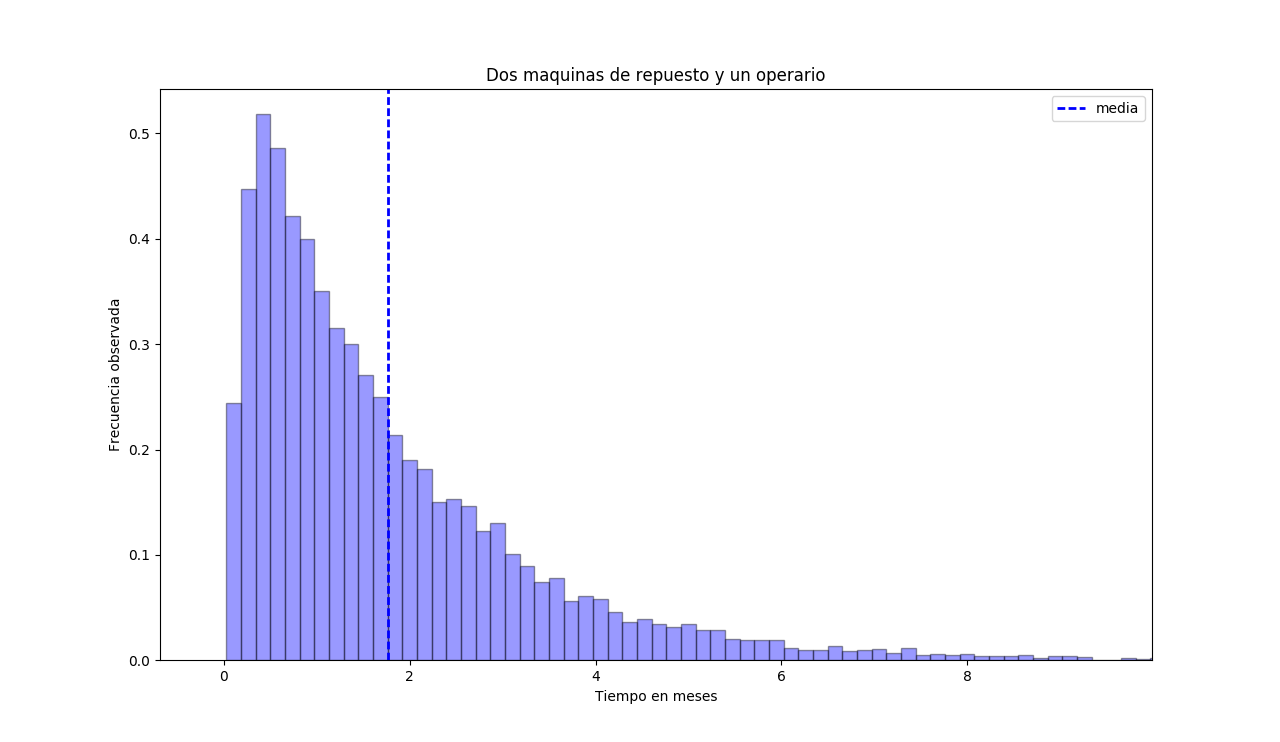
\includegraphics[scale=0.50]{1O2R.png}}
\centerline{$\mu= 01.7614$  \  $\sigma =1.6124$}
\end{figure}

Ahora veremos que conviene mas , si sumar un operario o agregar una nueva maquina de repuesto, en el caso de que se quiera aumentar el tiempo operativo medio del sistema. Para eso simularemos el sistema  con una maquina de repuesto mas , y  otra simulación con un operario mas. Considerando que  el tiempo de falla de la nueva maquina es igual a las que ya estan en el sistema y que el tiempo de reparación del nuevo operario es igual al del operario que ya esta trabajando.

\pagebreak

\subsection{Resultados de la simulación del sistema con 5 máquinas en uso, 2 máquinas de repuesto y 2 operarios}

\begin{figure}[hbt]
\noindent\makebox[\textwidth]{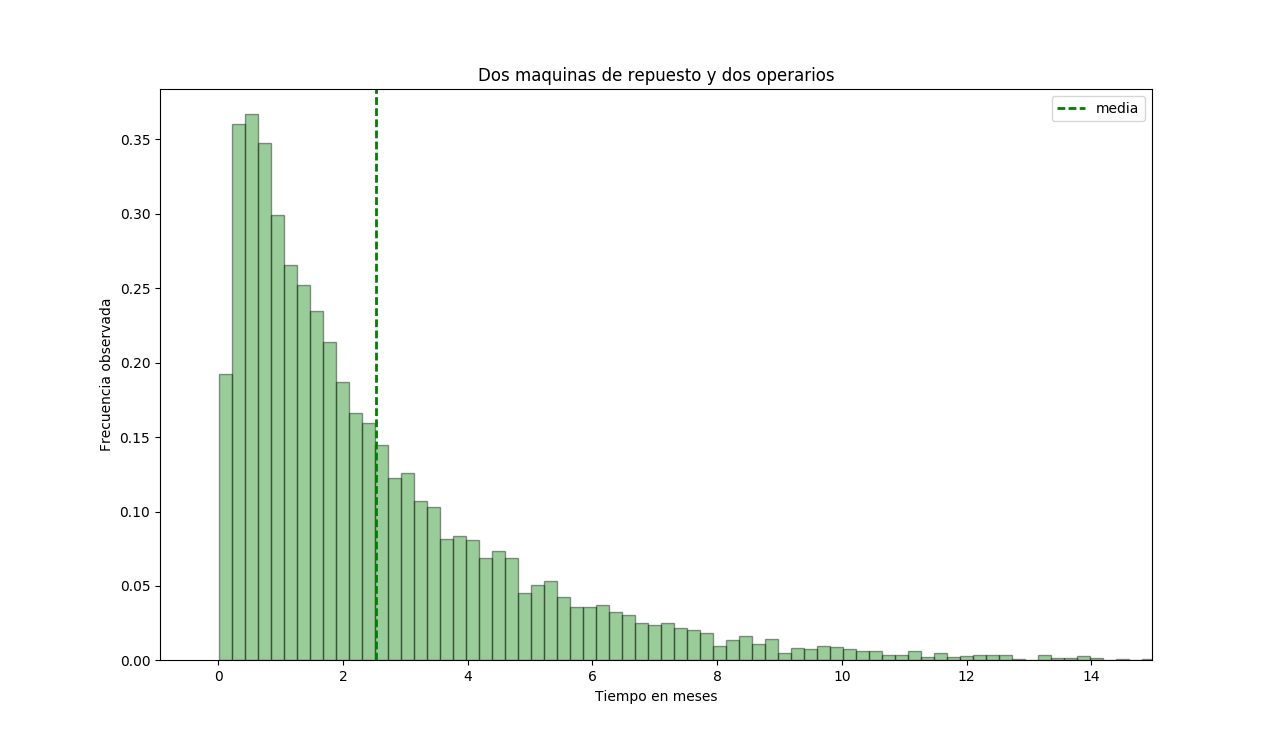
\includegraphics[scale=0.43]{2O2R.png}}
\centerline{$\mu= 2.5704$  \  $\sigma =2.4382$}

\end{figure}

Comparación entre el sistema original y el sistema con dos operarios: 

\begin{figure}[hbt]
\noindent\makebox[\textwidth]{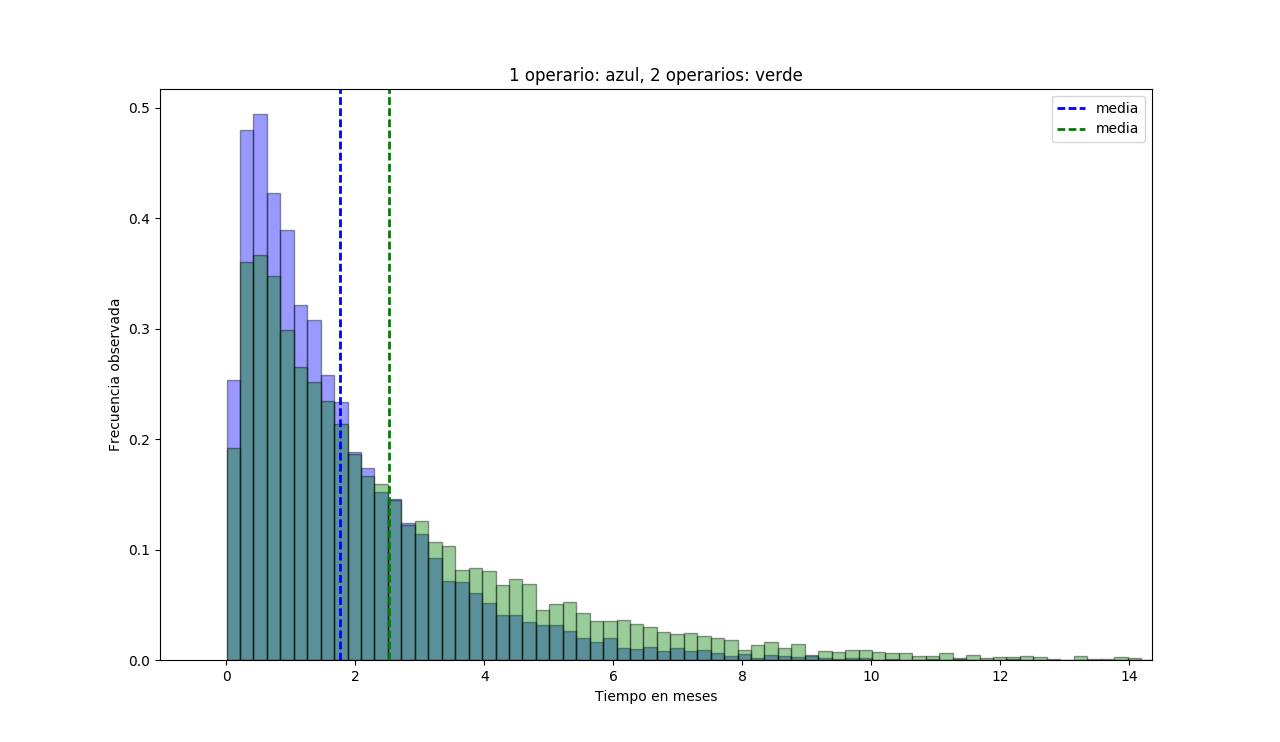
\includegraphics[scale=0.43]{1OS2y2OS2.png}}
\end{figure}

Como se puede observar en el grafico de arriba, al emplear un operario mas en el lavadero, se logra que en promedio, el lavadero puedo estar en funcionamiento por aproximadamente 0.8 meses mas.

\pagebreak

\subsection{Resultados de la simulación del sistema con 5 máquinas en uso, 3 maquinas de repuesto y 1 operario}

\begin{figure}[hbt]
\noindent\makebox[\textwidth]{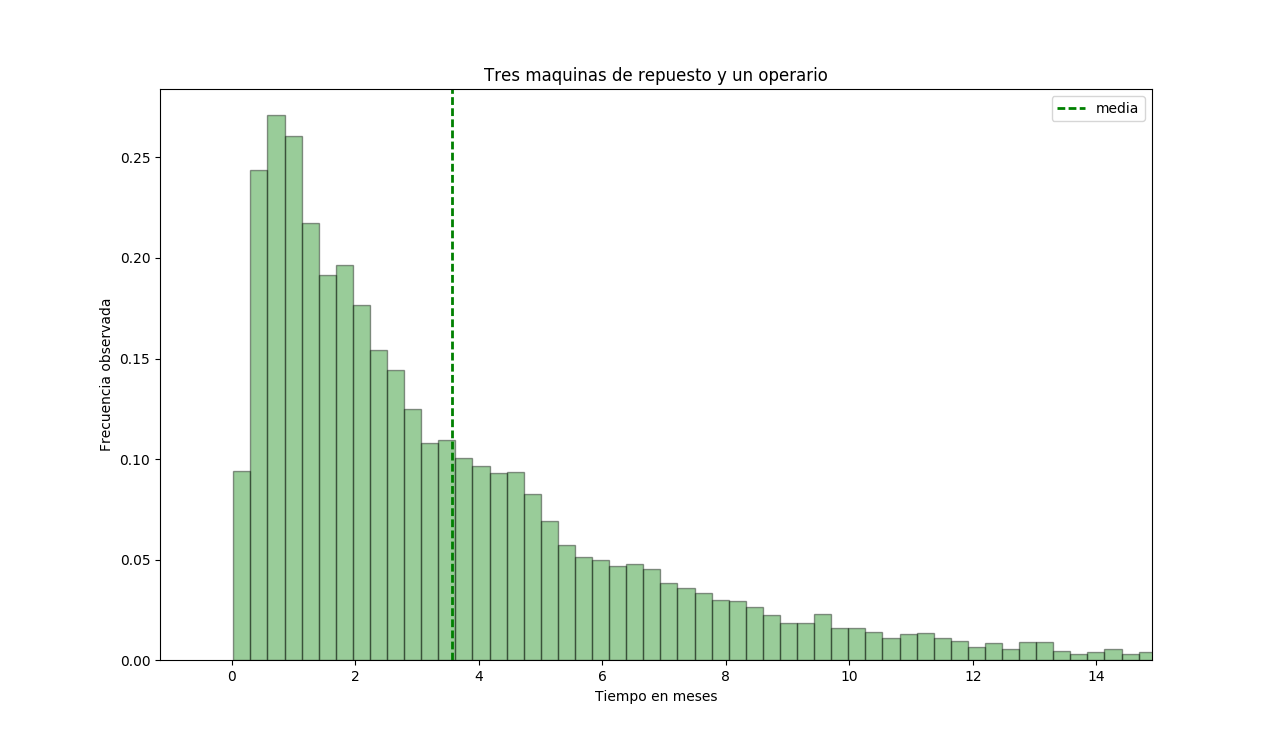
\includegraphics[scale=0.43]{1O3R.png}}
\centerline{$\mu= 3.5994$  \  $\sigma =3.2763$}

\end{figure}

Comparación entre el sistema original y el sistema con una máquina de repuesto mas: 

\begin{figure}[hbt]
\noindent\makebox[\textwidth]{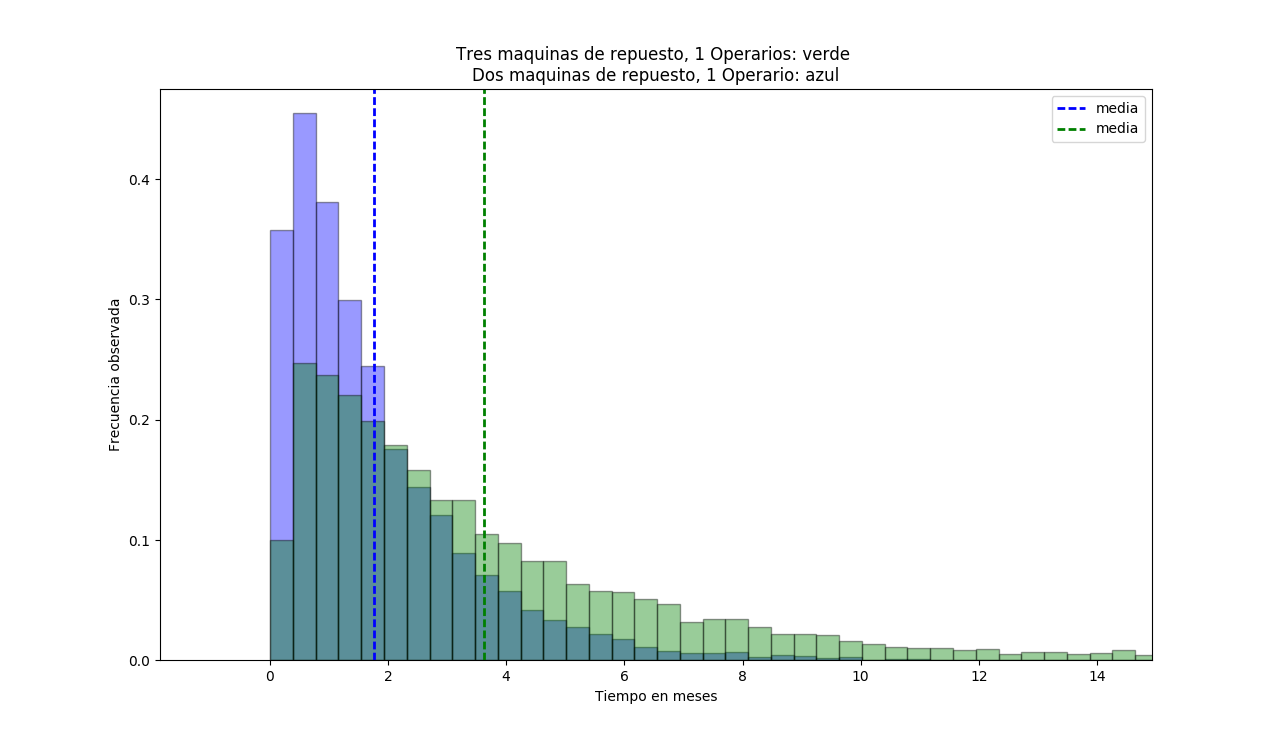
\includegraphics[scale=0.43]{1O3Ry1O2R.png}}
\end{figure}

En este caso la mejora con respecto al original seria aproximadamente de 1.84 meses.

\pagebreak

\subsection{Comparación de las mejoras del sistema}

El siguiente gráfico muestra la comparación entre las dos mejoras:

\begin{figure}[hbt]
\noindent\makebox[\textwidth]{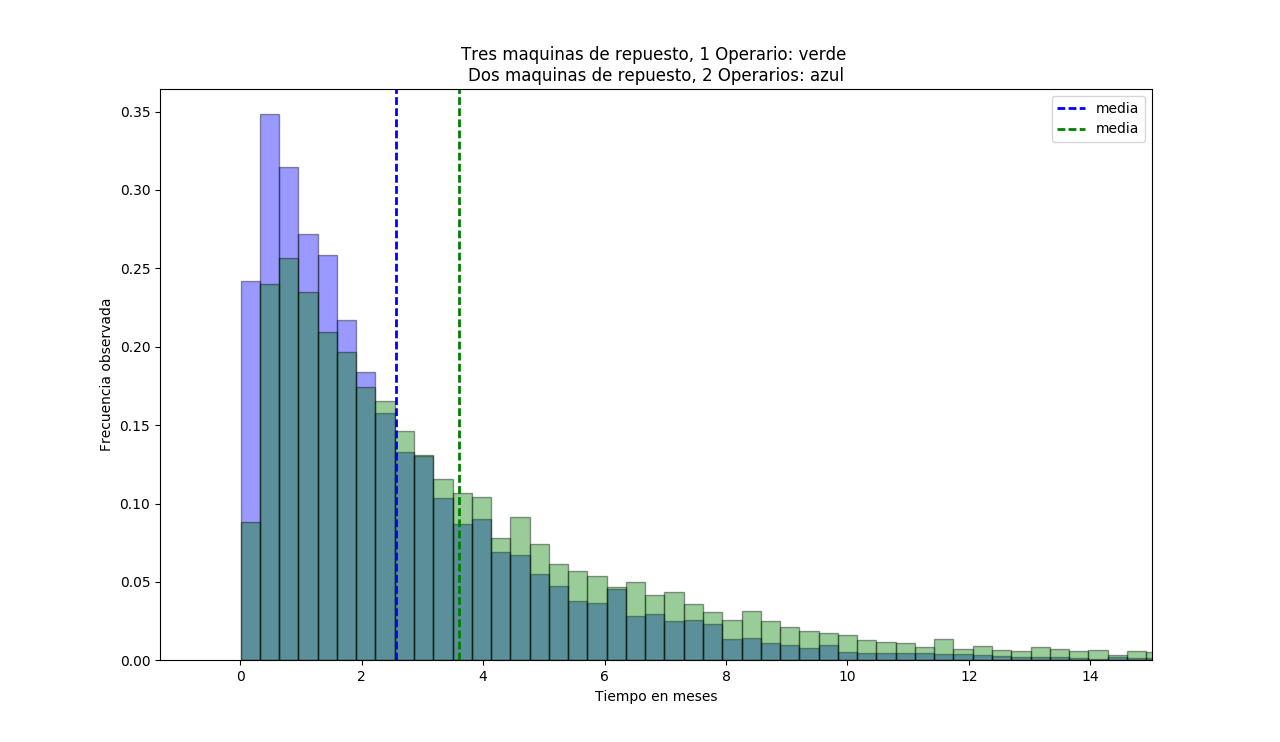
\includegraphics[scale=0.55]{1O3Ry2O2R.png}}
\end{figure}

Esta figura muestra que la mejora correspondiente a agregar una maquina es mas efectiva que la de agregar un operario.

\section{Conclusiones}
Finalmente la estimación que logramos mediante la simulación de 10000 fallos del sistema es que el tiempo operativo medio del sistema es $\mu=1.7614$  meses y su desviación estandar $\sigma=1.6124$, Ademas pudimos comprobar que para aumentar el tiempo operativo medio del sistema conviene agregar una maquina de repuesto ya que por la simulación estimamos que el tiempo medio seria $\mu=3.5994$ meses con esta mejora , en comparación con la simulación con un operario mas , que estimo un tiempo medio operativo de $\mu=2.570$.
  
\end{document}



cant_op=1 spare_machines=3
[3.5994256243586644, 10.734789677305239]
➜  cant_op=1 --spare_machines=2
[1.7614947402648904, 2.5998543210540457]
➜  cant_op=2 --spare_machines=2
[2.570493938173683, 5.945104722203743]
